\chapter{Il Network Slicing}\label{ch:capitolo1}

\section{Concetti principali}\label{ch:1.1}
La sempre più rapida evoluzione e innovazione delle tecnologie ha portato, negli anni, a modificare radicalmente le prestazioni ed i servizi richiesti alle infrastrutture di telecomunicazioni.\\
Internet, che ad oggi risulta la rete più diffusa al mondo, non rispecchia più le necessità  degli utilizzatori. Alla sua nascita, infatti, la Qualità del Servizio (QoS) richiesta era decisamente inferiore. Per questo motivo, la filosofia su cui è basato Internet è detta \textit{best-effort}: il sistema farà tutto il possibile per compiere un'operazione, ma non è garantito se e come questa sarà portata a termine.\\
Tuttavia, l'evoluzione di applicazioni e servizi ha reso necessaria una maggiore flessibilità delle prestazioni fornite dalla rete. A seconda dei casi, infatti, un servizio potrebbe richiedere bassa latenza, altri potrebbero avere bisogno di alto throughput. L'architettura e i protocolli di Internet non sono pensati per questo scopo e fornire prestazioni di questo tipo richiederebbe modifiche sostanziali.
\cite{libro1}\\
Da queste necessità nasce l'idea del Network Slicing.\\
Una \textit{Network slice} è un insieme di risorse che compongono una rete in grado di soddisfare le necessità di una specifica applicazione. Questo comportamento si può ottenere utilizzando diverse architetture e tecnologie che, insieme, ci permettono di manipolare il comportamento della rete.\\

\subsection{Software Defined Networking}\label{ch:1.1.1} 
Uno dei concetti alla base dell'idea del NS è il \textit{Software Defined Networking (SDN)}, ovvero la costruzione di reti in cui il \textit{routing} ed il \textit{forwarding} sono gestiti separatamente.\\
L'SDN prevede infatti la presenza di uno o più controller, che gestiscono il routing ed il comportamento complessivo della rete. I vantaggi che un approccio di questo tipo comporta sono molteplici.
\begin{itemize}
	
	\item La rete non è vincolata all'infrastruttura fisica. Il suo comportamento, definito via software, può quindi essere facilmente modificato e riprogrammato.
	
	\item La centralizzazione dell'intelligenza della rete stessa permette al gestore di operare solo sul controller, senza la necessità di intervenire su ogni singolo nodo. Inoltre, il controller permette di monitorare e supervisionare agevolmente l'intera infrastruttura \cite{6461195}	
	
\end{itemize}
\begin{figure}[h!]
	\centering
	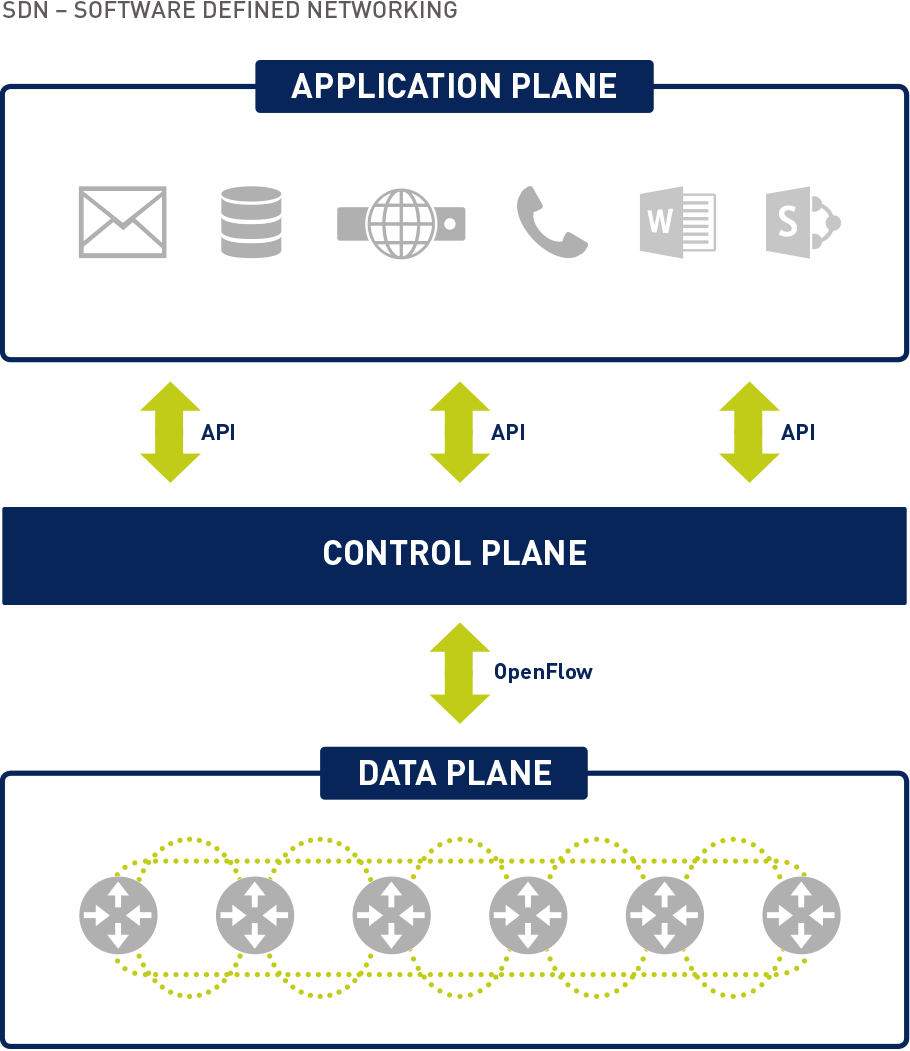
\includegraphics[width=0.6\linewidth]{../immagini/552578-sdn-graphic-blue-910}
	\caption[Software Defined Network]{Gestione software dell'infrastruttura fisica in una rete di tipo SDN}
	\label{fig:552578-sdn-graphic-blue-910}
\end{figure}

\subsection{Virtualized Network Functions}\label{ch:1.1.2}
Un altro elemento cardine per il Network Slicing è la \textit{virtualizzazione delle funzioni di rete (NFV)}. Le funzioni di rete, infatti, vengono solitamente implementate tramite hardware specifico in ogni nodo. Gli svantaggi di questa architettura includono l'alto prezzo dell'energia necessaria, un maggiore costo dovuto alla progettazione ed alla produzione dell'hardware stesso e l'inevitabile sempre più corto ciclo di vita di quest'ultimo.\\
La NFV si pone come obiettivo la soluzione di questi problemi, implementando le stesse funzioni di rete tramite software. Le \textit{funzioni di rete virtualizzate} non necessitano quindi di una specifica infrastruttura fisica, ma sono in grado di essere memorizzate ed eseguite da generici switch, server e data center, tramite la creazione su di essi di una o più macchine virtuali. Questo, insieme alla possibilità di poter spostare questi elementi hardware in qualunque nodo della rete, rende estremamente più pratica, economica ed efficiente la gestione della rete stessa. \cite{telecom_nfv}
\begin{figure}[h!]
	\centering
	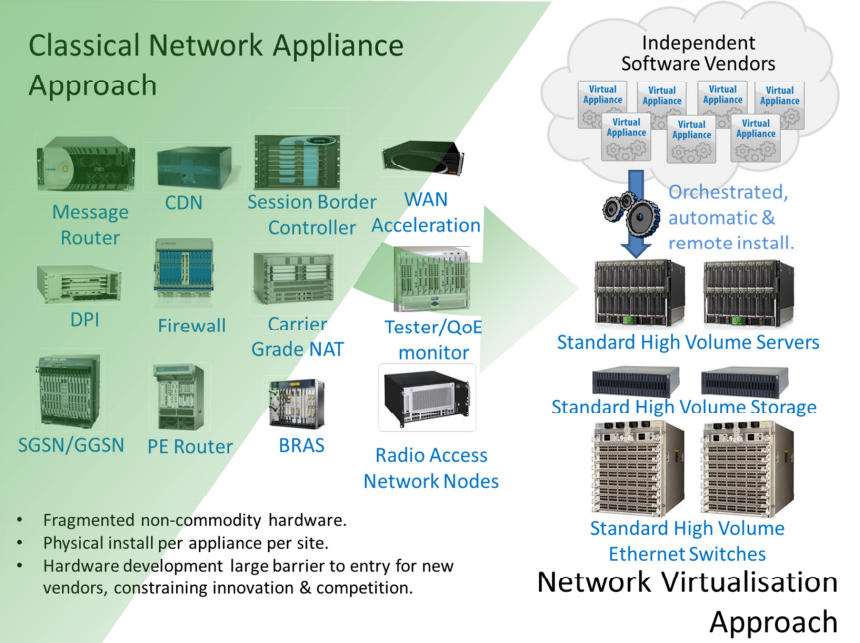
\includegraphics[width=0.8\linewidth]{../immagini/nfv}
	\caption[Network Function Virtualization, NFV]{Differenze tra l'hardware specifico richiesto normalmente dalle funzioni di rete e da quello generico utilizzato dalle VNF}
	\label{fig:nfv}
\end{figure}

\section{Architetture}\label{ch:1.2}
Lo scopo del Network Slicing è fare in modo che un'infrastruttura possa suddividere e organizzare le proprie risorse affinché un'applicazione abbia a disposizione una rete ottimizzata per le sue richieste.\\
Per fare ciò, queste architetture sono strutturate su 3 livelli:
\begin{itemize}
	
	\item \textit{Service Instance Layer}\\
	Rappresenta il servizio che deve essere supportato dalla rete. Ogni servizio è rappresentato da una Service Instance.
	
	\item \textit{Network Slice Instance Layer}\\
	Racchiude i vari Network Slices, ovvero le risorse allocate per una determinata Service Instance. Una Network Slice Instance può essere condivisa tra più SI.
	
	\item \textit{Resource Layer}\\
	Rappresenta le risorse e le funzioni di rete disponibili sull'infrastruttura, che verranno suddivise e assegnate in base al servizio richiesto.
	
	
\end{itemize}
L'intera architettura viene "orchestrata" da uno o più \textit{controller}, che hanno il compito di creare e organizzare le varie Istanze, stanziando le risorse necessarie per ciascun servizio.
\cite{NSintro}
\begin{figure}
	\centering
	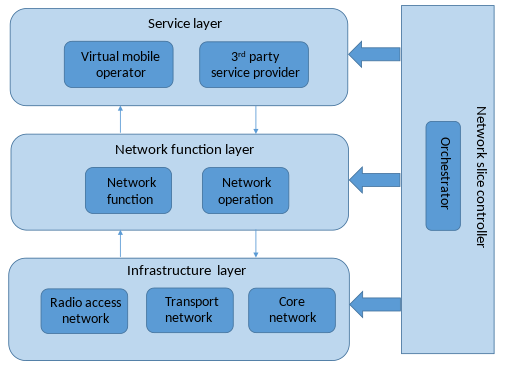
\includegraphics[width=0.9\linewidth]{../immagini/510px-Generic_5G_network_slicing_framework.svg}
	\caption[Architettura Network Slicing]{Struttura delle architetture di rete basate sul Network Slicing}
	\label{fig:510px-generic5gnetworkslicingframework}
\end{figure}\\
L'utilizzo di un solo controller può costituire un collo di bottiglia per le prestazioni della rete in caso di compiti particolarmente complessi. Per questo motivo può risultare efficace dividere i compiti tra più controller, assegnando a ciascuno la gestione di determinate funzionalità.
\begin{figure}
	\centering
	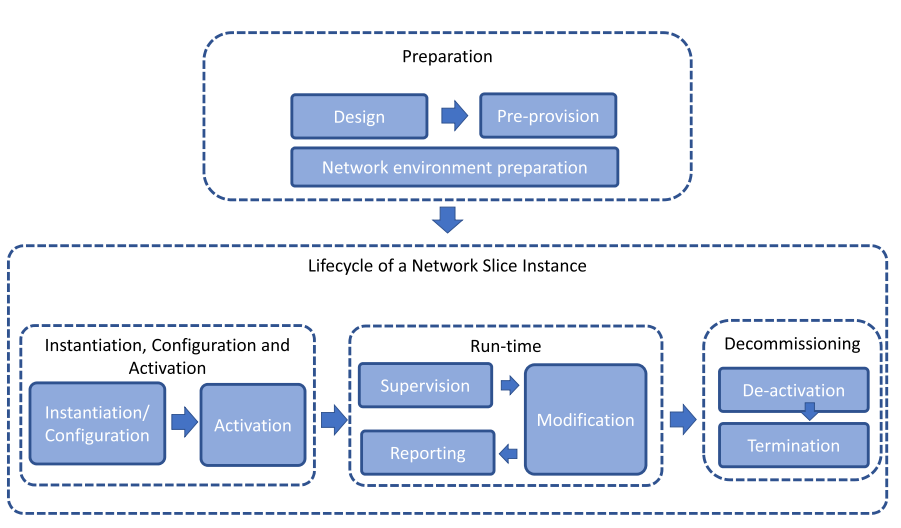
\includegraphics[width=1\linewidth]{../immagini/nslc}
	\caption[Network Slice life cycle]{Life Cycle di una Network Slice Instance}
	\label{fig:nslc}
\end{figure}\\\\
Il processo di creazione di un'Istanza inizia con un'operazione di progettazione e preparazione della stessa. Viene poi effettuata una richiesta di creazione, e attivazione della Slice. Una volta attivata, questa viene monitorata e modificata. Quando non è più necessaria, infine, viene disattivata e le risorse vengono rese nuovamente disponibili.\\\\
È importante sottolineare come le Slices siano tra loro isolate. Questo è un criterio fondamentale, che permette una maggiore privacy, impedendo di accedere ai dati delle altre Slices, e garantisce che le prestazioni di una Slice non influiscano sulle altre.\\\\
Il Network Slicing può essere implementato  in diversi modi. Un'infrastruttura con un unico proprietario avrà una gestione diversa rispetto ad una condivisa. Allo stesso modo, a seconda delle necessità, potrebbero essere necessari più o meno controller per gestire la rete.
\begin{itemize}
	
	\item \textbf{Singolo Proprietario, singolo controller}\\
	Questo è il caso più semplice, applicabile a porzioni ristrette della rete. In un'architettura di questo genere il Controller ha il compito di orchestrare direttamente l'infrastruttura e controllare direttamente tutte le Slices. Questo approccio può rappresentare un collo di bottiglia per l'affidabilità e per le prestazioni.
	\item \textbf{Singolo proprietario, più clienti}\\
	Quando risulta necessario aumentare il numero di quindi di controller, questi non possono più agire direttamente sulla rete. È infatti necessario inserire un intermediario tra di essi: questo ruolo viene svolto da un \textit{SDN proxy}, solitamente gestito dal proprietario della rete. Tra i vantaggi di questa architettura possiamo evidenziare la possibilità di permettere a vari utilizzatori di utilizzare i propri controller su un'infrastruttura fisica condivisa, mantenendo comunque l'isolamento tra le varie Istanze
	\item \textbf{Più proprietari}\\
	I precedenti casi sono riferiti a situazioni in cui l'infrastruttura fisica sottostante risulti sotto il controllo di un unico proprietario. Le Slices possono quindi essere composte semplicemente isolando e dividendo i rami della rete, assegnandoli alle varie Istanze.\\
	Tuttavia, nel caso in cui si vogliano utilizzare infrastrutture fisiche di proprietari diversi è necessario un ulteriore livello di astrazione, che permetta di rappresentarle come un'unica infrastruttura virtuale. Si crea così il concetto di \textit{rete virtuale programmabile}. \cite{libro1}\\
\end{itemize}
\begin{figure}
	\centering
	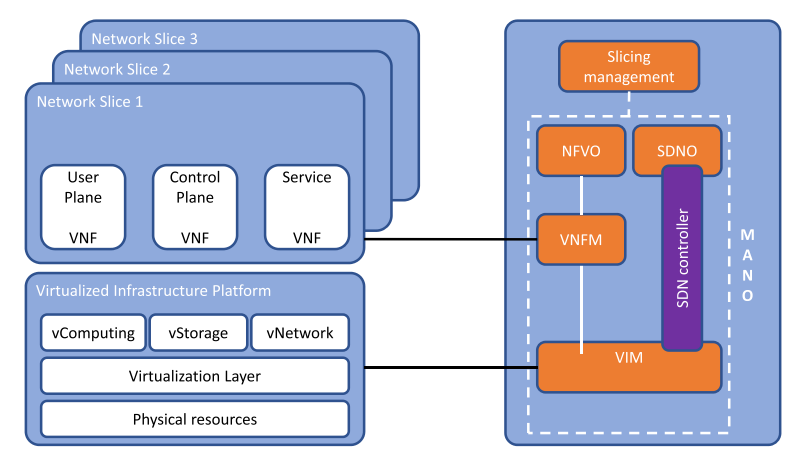
\includegraphics[width=0.9\linewidth]{../immagini/arch1}
	\caption[Architettura NS a singolo controller]{Struttura di un'architettura basata su Network Slicing a singolo proprietario e singolo controller}
	\label{fig:arch1}
\end{figure}
\begin{figure}
	\centering
	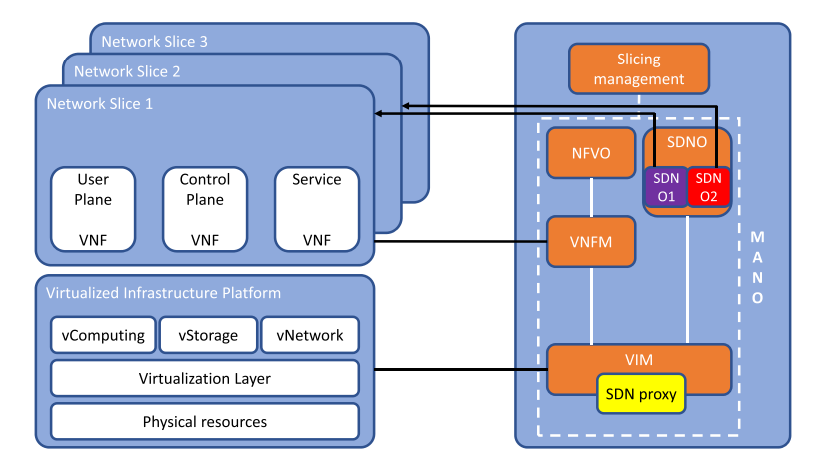
\includegraphics[width=0.9\linewidth]{../immagini/arch2}
	\caption[Architettura NS a doppio controller]{Struttura di un'architettura basata su Network Slicing a singolo proprietario e doppio controller}
	\label{fig:arch1}
\end{figure}

\section{Utilizzi e vantaggi}\label{ch:1.3}
L'idea del Network Slicing nasce con una strettissima correlazione con il 5G. Si prevede, infatti, che le reti di quinta generazione saranno in grado di creare grandi opportunità per nuove aziende e servizi. Questo porterà ad una grandissima varietà di richieste nei confronti della rete, che dovrà essere in grado di soddisfare necessità molto diverse tra loro.\\
Il Network Slicing si pone come una soluzione ideale a questo problema. La sua grande versatilità, infatti, risulta lo strumento perfetto per accontentare un'ampia gamma di richieste di varia natura. \cite{NS5g}\\\\
Queste tecnologie sono destinate ad innovare molte tipologie di comunicazione. Si prevede che un grosso impatto sarà percepito dall'industria e dai mercati verticali. Una rete flessibile e prestante ha infatti un'influenza significativa sulla produzione e permette di ottimizzare l'efficienza su tutti i livelli della filiera.\\
Un operatore può fornire al singolo cliente la gestione della propria Network Slice, permettendo di \textit{orchestrarla} a seconda delle proprie necessità. Un cliente può essere rappresentato da un'azienda che voglia basare la sua rete interna su un'infrastruttura di questo genere.\\\\
Tra i molteplici mercati che trarrebbero vantaggio da queste tecnologie possiamo evidenziare i seguenti.
\begin{itemize}
	\item \textbf{Automotive}\\
	La potenzialità più interessante delle telecomunicazioni nel campo dell'automotive è senza dubbio la comunicazione \textit{vehicle-to-everything}.\\
	Con questo termine si intende la possibilità di un veicolo di comunicare con diversi interlocutori in grado di fornire informazioni utili per comfort e sicurezza:
	\begin{itemize}
		\item L'\textit{Infotainment} è al giorno d'oggi una caratteristica imprescindibile di ogni veicolo. Una efficace comunicazione tra il veicolo e i passeggeri è fondamentale per una guida più attenta e confortevole.
		\item È opportuno anche che il veicolo sia in grado di comunicare continuamente con la casa madre, per mantenere il software e i dati sempre aggiornati.
		\item Per una maggiore sicurezza è importante garantire una comunicazione \textit{vehicle-to-vehicle} a bassissima latenza, per permettere di conoscere posizione e velocità reciproche e avere a disposizione un maggior numero possibile di dati riguardanti le condizioni della strada e del traffico.
		\item Sarebbe infine possibile offrire un'ulteriore sicurezza permettendo al veicolo di comunicare con vari sensori a terra in grado di monitorare traffico, visibilità o condizioni del manto stradale.
	\end{itemize}
	L'utilizzo per questo scopo di una rete pubblica 5g ottimizzata tramite Network Slicing permetterebbe di avere una maggiore copertura, maggiori prestazioni e un costo inferiore.
	
	\item \textbf{Energia}\\
	Una delle più importanti nuove frontiere nel campo dell'energia è rappresentata dalle \textit{Smart Grids}.\\Questo termine sta ad indicare una rete di distribuzione di energia supportata da un costante flusso di informazioni, in grado di gestire in maniera intelligente la distribuzione dell'elettricità, evitando sovraccarichi e minimizzando le perdite.\\Inoltre, con la diffusione degli impianti fotovoltaici privati, la rete deve essere in grado di convogliare adeguatamente al proprio interno l'energia prodotta.\\
	Un'infrastruttura che permetta queste operazioni al momento non esiste. Una rete 5g supportata dal Network Slicing sarebbe in grado di svolgere efficacemente queste funzioni, garantendo le prestazioni richieste.\\
	Le necessità di una rete in questo ambito sono una zona di copertura molto estesa, una bassa latenza e una grande affidabilità, anche in situazioni di emergenza.
	\begin{figure}
		\centering
		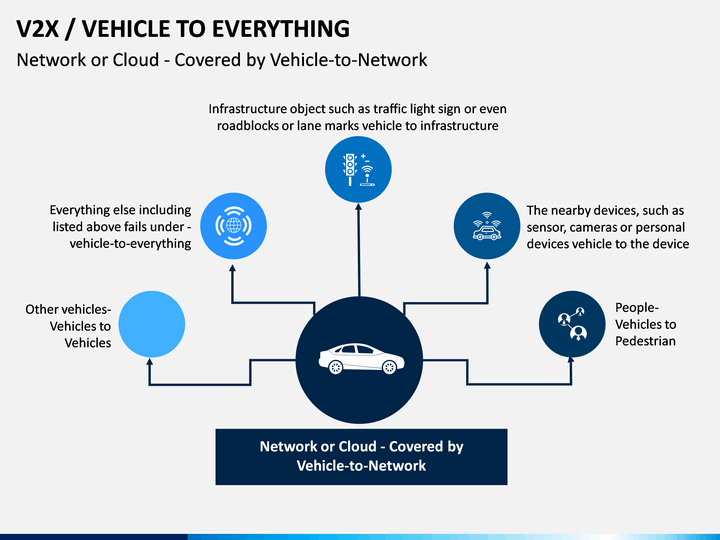
\includegraphics[width=0.75\linewidth]{../immagini/vehicle-to-everything-slide12}
		\caption[Vehicle-to-everything]{Comunicazioni di tipo Vehicle-to-Everything (V2X)}
		\label{fig:vehicle-to-everything-slide12}
	\end{figure}
	\begin{figure}
		\centering
		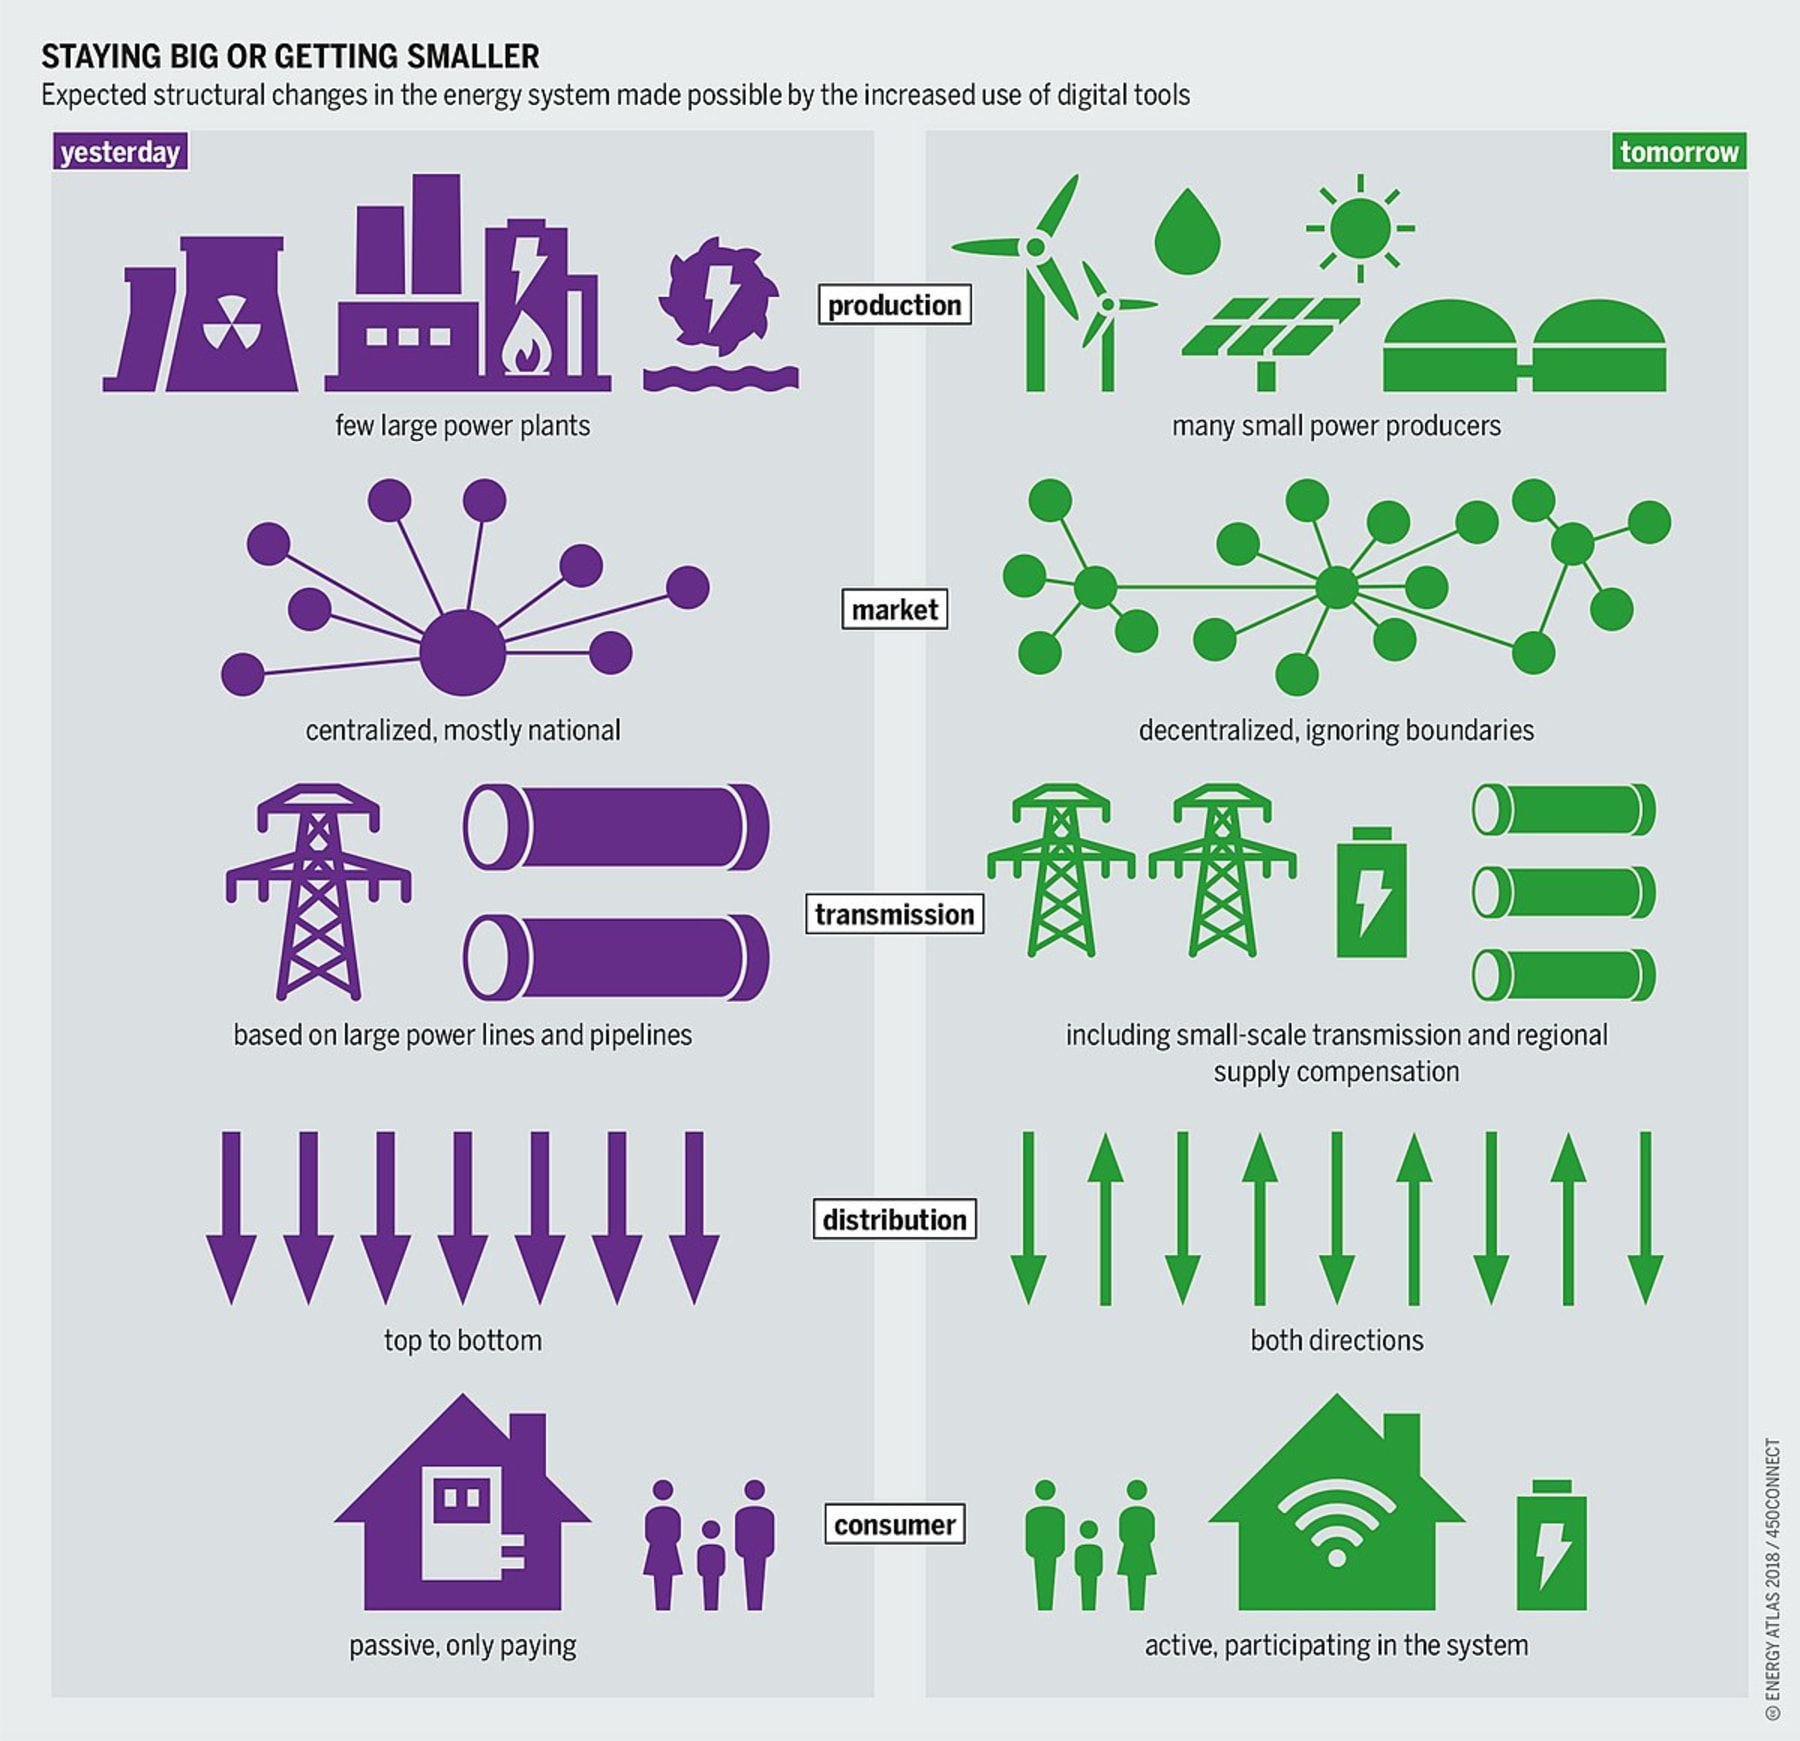
\includegraphics[width=0.75\linewidth]{../immagini/0_7i2ht2hZquYBwybh}
		\caption[Smart Grids]{Produzione e gestione dell'energia tramite Smart Grid, supportata da una rete di informazione}
		\label{fig:07i2ht2hzquybwybh}
	\end{figure}\\
	
	\item \textbf{Sanità}\\
	In ambito sanitario, l'implementazione di reti flessibili e prestanti aprirebbe tantissime opportunità.\\
	Una tra le novità sarebbe sicuramente la possibilità di monitorare in tempo reale le strumentazioni e i pazienti dentro e fuori gli ospedali.\\
	Tuttavia, risulta ancora più interessante l'idea della \textit{chirurgia da remoto}. Avere a disposizione una rete in grado di fornire una bassissima latenza, infatti, permetterebbe ai chirurghi di operare pazienti senza essere fisicamente in ospedale. Questo risulterebbe fondamentale in caso di operazioni specialistiche eseguite da esperti, riducendo drasticamente i costi per i pazienti ed eventualmente salvandone la vita.
	
	\item \textbf{IoT e Smart Cities}\\
	IoT e Smart Cities sono campi in continua espansione, per i quali una connessione su aree di grandi dimensioni risulta fondamentale. L'idea di base è di avere una vasta rete di sensori che permettano di raccogliere dati e gestire di conseguenza svariati parametri, come illuminazione o riscaldamento, in modo da avere un funzionamento ottimale e minimizzare i consumi.\\A differenza delle applicazioni precedentemente citate, la latenza non è un requisito stringente. È tuttavia fondamentale che i vari elementi della rete abbiano un basso dispendio energetico e che la copertura sia sufficiente a garantire che tutti i sensori possano comunicare.  \cite{5g5}\\
	
\end{itemize}I vantaggi apportati dal Network Slicing sono quindi numerosi e di diversa natura, a seconda del servizio richiesto e della necessità del consumatore.\\\\
Nel capitolo 3 verranno confrontate le prestazioni di una rete classica con quelle di una rete costruita seguendo i principi del Network Slicing.